% ****** Start of file apssamp.tex ******
%
%   This file is part of the APS files in the REVTeX 4.1 distribution.
%   Version 4.1r of REVTeX, August 2010
%
%   Copyright (c) 2009, 2010 The American Physical Society.
%
%   See the REVTeX 4 README file for restrictions and more information.
%
% TeX'ing this file requires that you have AMS-LaTeX 2.0 installed
% as well as the rest of the prerequisites for REVTeX 4.1
%
% See the REVTeX 4 README file
% It also requires running BibTeX. The commands are as follows:
%
%  1)  latex apssamp.tex
%  2)  bibtex apssamp
%  3)  latex apssamp.tex
%  4)  latex apssamp.tex
%
\documentclass[reprint,amsmath,amssymb,aps]{revtex4-1}

\usepackage{graphicx}% Include figure files
\usepackage{subcaption}
\usepackage[hidelinks]{hyperref}
\usepackage{dcolumn}% Align table columns on decimal point
\usepackage{bm}% bold math
\usepackage[british]{babel}
%\usepackage{hyperref}% add hypertext capabilities
%\usepackage[mathlines]{lineno}% Enable numbering of text and display math
%\linenumbers\relax % Commence numbering lines

%\usepackage[showframe,%Uncomment any one of the following lines to test 
%%scale=0.7, marginratio={1:1, 2:3}, ignoreall,% default settings
%%text={7in,10in},centering,
%%margin=1.5in,
%%total={6.5in,8.75in}, top=1.2in, left=0.9in, includefoot,
%%height=10in,a5paper,hmargin={3cm,0.8in},
%]{geometry}

\begin{document}

\preprint{APS/123-QED}

\title{Microplatforms: Product platforms as code}% Force line breaks with \\

\author{Stuart Harris}
\email{stuart.harris@red-badger.com}
\author{Viktor Charypar}%
\email{viktor.charypar@red-badger.com}
\affiliation{Red Badger Consulting Ltd.}

\date{\today}

\begin{abstract}
Microplatforms are an automation-based approach of provisioning and operating platforms to run digital products and services, which emphasises autonomy of cross-functional product teams. We discuss the traditional approach of building a large-scale, shared platform and explore the resulting cost to the organisation, chief of which is the cost of coordination between teams. Instead, we offer the concept of each cross-functional team owning and operating a separate, self-contained platform. A key enabler for this approach is full automation - capturing all aspects of the product and the platform from provisioning to service orchestration and policy as source code. This approach results in significantly increased team autonomy and enables agile architecture, continuous deployment to production and ongoing innovation. Microplatforms allow organisations to move engineering effort higher up the value chain and focus on using technology to solve customer problems.
\end{abstract}

\maketitle

%\tableofcontents

\section*{Introduction}
\label{sec:introduction}

When building and delivering a real-world client-server application or service, it is important to consider all the parts that form the product, and without which the product would not operate. Typically we think of the product as two major components - the application itself and the platform it runs on. However, there are many other tools, processes, activities and concerns involved in delivering a Software as a Service (SaaS) product to its users than is covered by the functional features and the runtime environment alone (See figure \ref{fig:concerns}).

\begin{figure}[b]
	\setlength{\fboxsep}{1em}
	\fbox{
		\begin{minipage}{0.43\textwidth}\raggedright
			Service name, Programming language(s), Programming paradigm(s), Architectural choices, Integration pattern(s), Transport protocols, Authentication, Authorization, Reporting, ETLs, Databases, Caching, Platform libraries, Service dependencies, CI Pipeline dependencies, 3rd party library dependencies, 3rd party service dependencies, Security threat model, License audit, Compliance audit, Capacity plan, Provisioning plan, Cost reporting plan, Monitoring plan, Maintenance process, Backup and Restore process, Secret management, Secret rotation, On-Call schedule, Configuration management, Workflow management, Alerts, Log aggregation, Unhandled failure aggregation, Operations and incident response runbooks, API documentation, Source Code Repository, Humane Service Registry, Service Discovery Registry, Distributed Tracing Registry, Monitoring Dashboard Registry, Build Artifact Repository, CI pipeline(s): Build, Test, Publish, Integration tests, Contract tests, Canary, Deploy, Post deploy tests.
		\end{minipage}
	}
	\caption{48 concerns for a single microservice~\cite{Treadway17:online}}
	\label{fig:concerns}
\end{figure}

Starting with the software itself, it is crucial that it is thoroughly tested before any part of it can be considered done. Testing is now typically largely automated~\cite{TestPyra22:online}, although manual exploratory testing is also strongly advised~\cite{Explorat86:online}. Testing activities fit on a scale of the level of integration of all the components involved, from testing each in isolation (e.g. unit testing) to fully integrated testing of the run-time behaviour of the entire application stack.

Typically, this is supported by a number of different environments~\cite{Professi40:online} starting from the lower ones, where external dependencies of services are stubbed~\cite{TestStub82:online} and moving all the way up to the production environment which serves customers. Traditionally, these environments are named, long-lived, and are often reused for the purposes of various different testing activities (e.g. functional, performance, and penetration testing).

In order to get applications deployed, configured and started in these environments a process of deployment activities is followed, ranging from completely manual to fully automated. There are several different methodologies addressing the change-related risk of deploying to the production environment, ranging from large regular deployments done every few months all the way to Continuous Delivery and Continuous Deployment~\cite{WhatisCo44:online}.

Continuous Deployment is a method in which every change to the codebase gets deployed immediately, which necessitates a fully automated process of testing and deployment, in order to reduce the risk of human error and speed the process up enough so that it doesn’t dominate all the development activities. The result has the benefit of deploying smaller increments, which have far smaller impact when things go wrong, and significantly reduces the scope of diagnosing the failure and the time to recovery. Delivering product in smaller increments also reduces time to market with the first increment already providing value and customer feedback (and potentially generating revenue), while the rest is being developed.

Typically, when following the continuous deployment method, businesses do not want customers to immediately see the change caused by every deployment and so mechanisms such as feature flags~\cite{FeatureT95:online} are introduced in order to decouple deployment of code changes from releases of customer functionality. This has numerous benefits for both sides, since the ability to release is no longer dependent on the ability to deploy and vice versa.

A platform supporting a digital product which is available to customers any time of day, seven days a week also has to have the ability to tolerate failure of infrastructure or individual components without failure of the product itself. This is commonly referred to as high-availability~\cite{HighAvai70:online} and is generally achieved by running several instances of the same services spread across geographical locations, so that the application can keep working even when an entire data center is lost. This horizontal replication is also used for scaling the application with customer demand~\cite{WhatIsAm85:online}.

An important consideration for a product platform is the cost of building it and the ongoing maintenance involved, including infrastructure provisioning, maintenance (security patches) and scaling capacity to support the products that need to run on it. The effort involved should not be under-estimated~\cite{saaspdf24:online} and is the motivation behind most digital product now running on cloud infrastructure. We will discuss the reasons for this cost reduction in more detail in sections~\ref{sec:cost} and~\ref{sec:automation}.

Finally, a product platform needs to include features supporting the constraints of running digital products in safety-critical or regulated environments, e.g. medicine or finance. This means supporting information security features (e.g. secure secrets management for credentials), role based access control with good identity and access management~\cite{RoleBase56:online} and full audit trail and other controls necessary to reduce the risks involved in all of the activities described above.

There has been a clear trend over the past two decades of automating as much of the above activities as possible and treating them as another part of the product itself. This is the core proposition of cloud services and a key concept of the DevOps movement~\cite{DevOpsCu34:online}.

In this paper we will investigate ways of leveraging automation to design, build and manage everything involved in building and deploying digital product to the level where the entire product platform can be fully owned by a small, cross-functional product delivery team, enabling significantly increased capability and velocity of product delivery.

In section \ref{sec:benefits} we outline the goals a good product platform should aim to support. In section \ref{sec:cost} the current approach of using a shared platform is discussed and an alternative (Microplatforms) is suggested in section \ref{sec:microplatforms}, supported by the concept of managing all aspects of it as source code in section \ref{sec:ascode}. Finally, we describe a reference architecture of an example Microplatform in Appendix~\ref{sec:architecture}.


\section{Benefits provided by a product platform}
\label{sec:benefits}

A product platform should ideally support several goals of the organisation in order to realise return on the investment of designing and building it in the first place. The main benefit of a product platform should be reducing the time spent on manual operational tasks, deployments and testing, ultimately translating to increased reliability and greater velocity of the teams. A platform should support the cross-functional team in practicing DevOps: building the product features and delivering them to customers quickly and with minimum risk of causing defects or outages.

The goal of Agile software delivery methodologies like Lean~\cite{LeanSoft20:online} is to eliminate all waste from the process, thus increasing throughput. Focusing on the platform, the waste can be in, for example, being impeded by platform downtime, working around (missing) platform features, repeatedly performing manual tasks or coordinating with other teams to perform tasks (we will discuss the coordination costs in the next section in more detail).

Deployment of code should be automated and the platform should support practices that reduce or eliminate the risks involved (e.g. techniques like rolling updates~\cite{Performi30:online}, blue-green deployments~\cite{BlueGree26:online}, canary releases~\cite{CanaryRe28:online}, etc.). Regression testing should also be automated and be reliable enough to make it virtually impossible to deploy a broken application. This automation ultimately enables continuous delivery of customer value as an overarching goal to gain the ability to rapidly improve the product based on real customer behaviour~\cite{Continuo59:online}.

The platform also needs to provide good support for the chosen architecture of the application itself. The currently accepted best practice for medium to large scale systems is Microservices Architecture~\cite{Microser99:online}, which provides numerous benefits for modularity and scalability of the overall solution, but comes with its own set of difficulties in managing the orchestration of a large number of microservices that need to work together as a system. The platform should support this approach with service discovery and configuration management features and reduce the overhead that managing microservice orchestration generally involves.

In the long term, the platform should be flexible enough to support safe technical innovation in all directions and enable practices like evolutionary architecture~\cite{Microser21:online} and continuous improvement~\cite{KaizenTh68:online} even for the infrastructure. We will refer to these features using the term \textit{Agile Infrastructure}. Having the ability to evolve the infrastructure design eliminates the need for large up-front planning and enables ongoing innovation in a way that is similar to Agile software delivery.

Finally, the platform should have built-in features to support information security - prevent intrusions and minimise their impact if they cannot be prevented - and compliance with internal and external regulation that can be easily demonstrated. At a bare minimum, the platform should have access control features and full auditability support. Ideally, it should also be agnostic of the underlying infrastructure provider in order to avoid vendor lock-in and allow the platform to be portable if needed.


\section{The cost of a shared product platform}
\label{sec:cost}

Given the goals and required features listed in the previous section, it should be no surprise that designing and building a product platform for a medium to large organisation with many products and product teams involves a large investment of resources and time. The obvious, and thus far the only way of offsetting this cost is to build a single large product platform shared by all the product teams [refs - google, facebook...]. The cost of building a product platform generally breaks down into two parts - the one-time upfront cost and the ongoing cost.

The initial investment involves the design, building, stabilising and scaling of the platform, typically done manually in the past, i.e. provisioning servers on premise or in the cloud, configuring them, linking them into HA clusters, setting up networking, etc. This requires specialist skills typically leading to the formation of a platform engineering team []. The cost of this initial phase always ends up significantly more than expected, understood or attributed.

Sharing the platform implicitly requires multi-tenancy features, e.g. the concept of organisations and projects, granular role-based access control, resource limits and isolation, etc. Moreover, in order for the platform to be shared by all teams, the feature set needs to be a union of all the features required by each team. In the theoretical extreme cases, this means supporting $n$ disjoint sets of features for $n$ teams, or forcing all the teams to use the single set of features prescribed by the platform.

The former extreme is very costly to scale and requires a lot of engineering effort to support, while the latter limits the product team’s ability to deliver exactly what is needed by the customer, as the team has to work around decisions made by someone else (and for someone else). This is an example of the 80/20 rule where a shared platform will get you 80\% of the way very easily and the rest becomes a significant challenge, which just ends up frustrating the efforts of the team and the business.

Overall the feature set of a shared platform ends up significantly larger than the set of features required by a single team, increasing the cost and complexity of the platform. The pressure to reduce this cost to a manageable level often leads to limitations for individual product teams requiring niche features that were dropped out of scope.

After the initial build is completed, more investment needs to be made on an ongoing basis to run operations, i.e. provision new hardware, patch operating systems with fixes, add more resources, clean up older instances of services, etc. In order to serve the business for several years, new features need to be added as they become available in the industry in order to stay within the recognised best practice (often referred to as evergreening).

By far the largest ongoing cost to the business, which is often not explicitly recognised, is the cost of coordination between the product teams and the platform engineering team. Unless every common task from provisioning and getting access to regular deployments and elastic scaling is automated, the product teams need to ask for help from the platform team. The platform team quickly forms a large backlog of day to day tasks to perform, product teams end up queueing behind others, and the platform team have much less time to invest into improvements of the platform itself and automation of the daily tasks.

In large organisations, the team structure is typically much more complex, forcing the platform team to request help from other teams, like, for example, IT infrastructure, IT security, networking, etc. amplifying the slow-down even further. This results in a situation sketched in figure \ref{fig:dependencies}, where each product team has several dependencies on solution delivery teams, each of which have multiple different customers and often depend on each other as well.


\begin{figure}[h]
	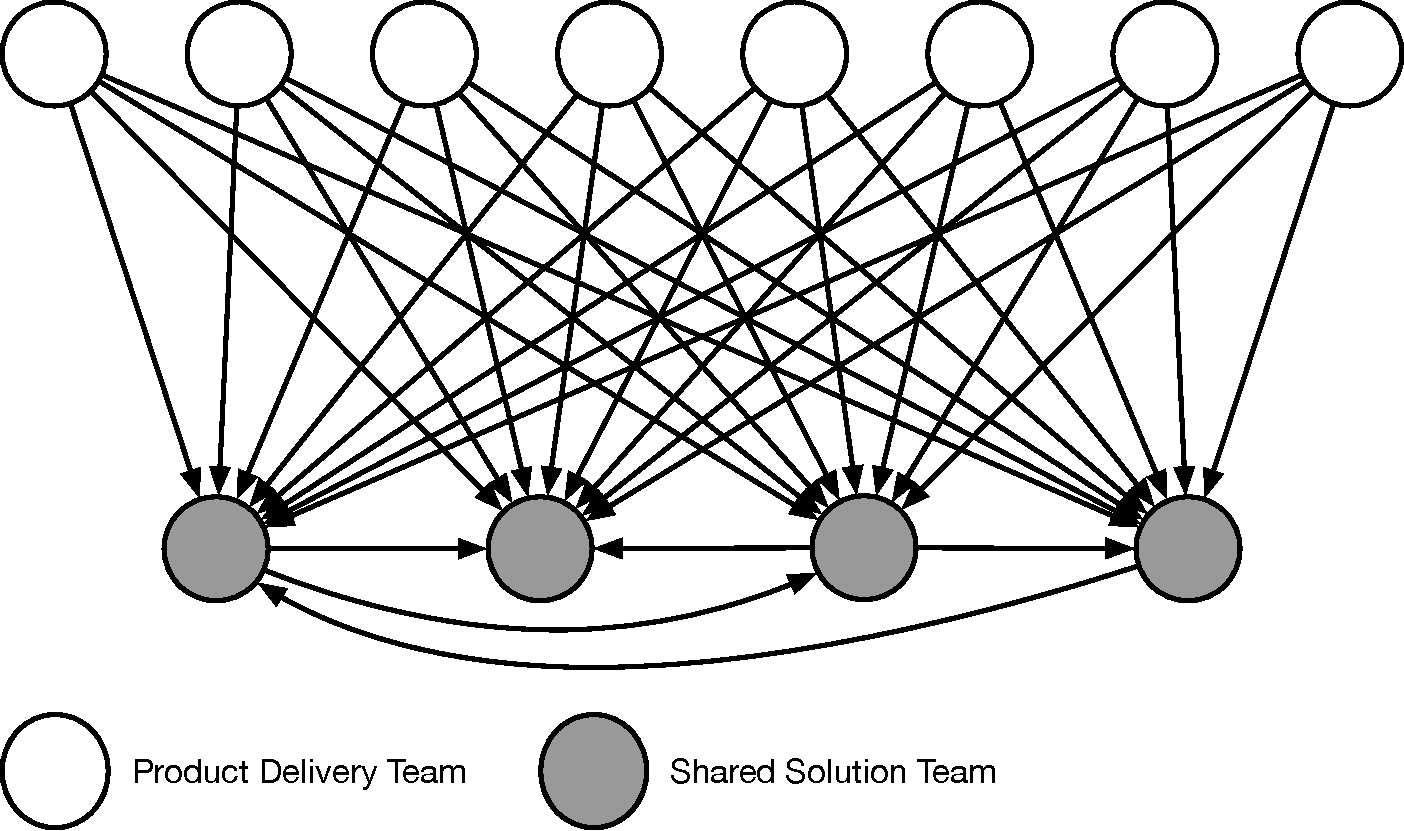
\includegraphics[width=0.45\textwidth]{figs/dependencies}
	\caption{Team dependency structure with shared solution teams}
	\label{fig:dependencies}
\end{figure}

The impact of this effect, especially in the early stages of building a shared platform is so significant, it can cause the entire project to fail completely (since it is no longer helping the product teams deliver value to customers, it is now taking away from that ability), unless the platform team has significant resources to withstand this pressure.

The overall cost of building and operating a shared product platform is large enough to pose a serious risk to the business. Typically, when things do not go well, this leads to resistance to cut the losses - the sunk cost fallacy~\cite{TheSunkC23:online}. Instead of trying again, or exploring different solutions, the attitude turns into “we will make it work” and results in products being built on a mediocre platform with reliability and scaling issues, increasing risk of preventable outages and slowing down product delivery. This is the final, often unrecognised, cost of a shared product platform - the missed opportunity cost of not delivering as much customer value as possible.

Even when things go well, the size of the investment means that when, eventually, the time comes to abandon the current platform in order to innovate using the latest available technology, nobody is willing to make the investment again, even though it could bring an order of magnitude improvement in efficiency of software delivery. This could be described as technology lock-in or a solution lock-in (similar to vendor lock-in []) - with a large-scale platform build, the required investment is so large that a single organisation is not likely to get a return on investment before the need to iterate on technology choices appears because the pace of technical innovation in the industry is so rapid.

It may seem like the only option left is to not spend the effort of building a shared platform in the first place and instead reach for a solution available in one of the cloud vendor offerings. This reduces the cost of building and scaling the platform, but the cost of sharing and the risk of lock-in stays. Further, the organisation is no longer fully in control of the available tools or the way they are being used by the teams and as a result, most organisations opt for some form of governance around the cloud offering as well, which effectively leads to the same situation as the custom build in terms of coordination cost, and the limited, centrally managed set of available features. Moving to a cloud native solution seems to treat some of the symptoms of the problem, but it does not cure the underlying cause, nor does it guarantee the end result will be any more fit for purpose.

The common theme and, in our opinion, the underlying source of the shared platform costs is the fact they are \textit{shared} among a relatively large number of different product teams. (Notice that the problems listed above seem much less significant if you imagine the platform is only supporting three product teams). The shared nature is what leads to the need for the extra features that enable the sharing, it is also the source of scaling and reliability challenges and, most significantly leads to the rise of coordination costs.

Given the above, our goal should be to enable as much product team autonomy as possible, removing all of the incidental dependencies that are not part the business or customer problem being solved, but rather are created by the solution that has been chosen (often without involving the product delivery team). With a better informed choice of solution, instead of solving the incidental problems and making incidental dependencies more efficient, we can simply make the problems not occur in the first place and remove the dependencies entirely.

The ideal situation would therefore be for each product team to be fully in control of their entire product - the application, the platform, the entire life-cycle and everything described in section \ref{sec:benefits}. The only shared dependencies left are the essential ones that have to be shared, i.e. sharing them brings clear benefits (e.g. central systems of record, single sign-on identity providers, source control repositories, artefact registry, etc.). In order for this approach to be practical in a small agile team and safe in the context of a large organisation, we need to leverage as much automation as possible.


\section{The rise of automation}
\label{sec:automation}

In the previous section, we covered the level of effort and the number of people necessary to build a product platform. This, however, is largely a result of building and configuring infrastructure manually. Provisioning and setting up servers, clusters, networks and systems by hand requires a large amount of effort and the complexity and difference of individual tasks involved requires specialisation, requiring yet more people.

\begin{figure}[h]
	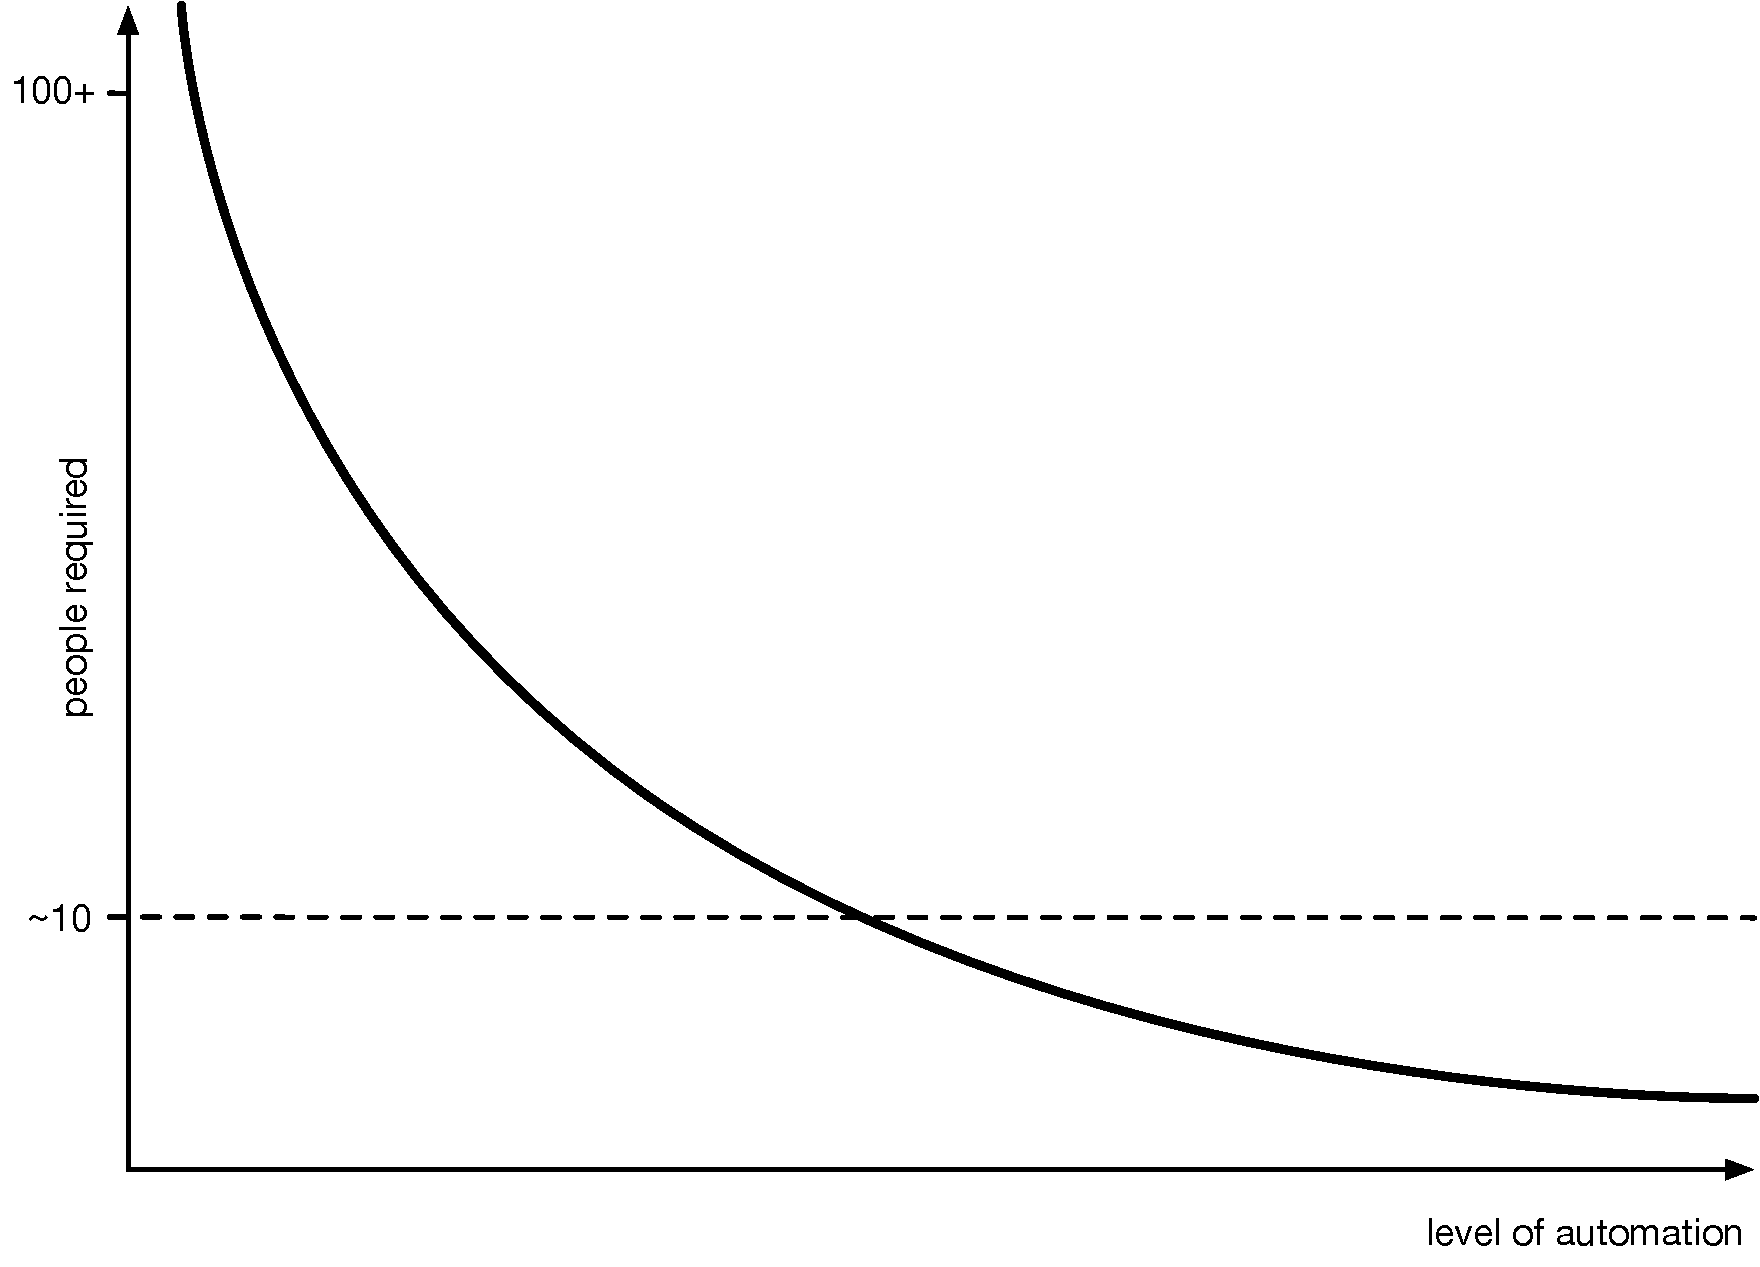
\includegraphics[width=0.45\textwidth]{figs/automation}
	\caption{Effect of automation}
	\label{fig:automationn}
\end{figure}

Fortunately, as software engineers, we know the way out of this problem: encoding the repetitive tasks (even the ones that require a specialist) in automation. Simplifying a little bit, as more and more tasks are automated, fewer and fewer people and less specialisation is required (figure \ref{fig:automationn}).

This is not a new finding, automating certain tasks is an accepted practice in multiple industries including software engineering. An obvious example is regression testing using automated unit tests, integration tests and end-to-end tests. Testing used to be a manual task performed by humans following test scripts. Automating it significantly decreased the time between deployments allowing us to get from deploying every few months to several times a day, enabling a completely new working practice known as Continuous Deployment to Production (CDP). This decreases risk of deployments to a minimum due to the size of deployments and reliability of the process. It also minimises mean time to recovery from incidents (requiring a code change to resolve), and results in an overall increase in reliability and a leap in both delivery velocity and ability to adapt to customer needs.

Similarly, the success of cloud services is in a huge part down to allowing automation. Instead of spending weeks manually provisioning servers and network infrastructure, the same infrastructure can be provisioned automatically within minutes. Leveraging cloud services, a small team of engineers can set up a web or mobile application infrastructure that will vastly outperform one set up manually (over weeks or months) by a traditional IT organisation in every measure. [ref?]

\begin{figure}[h]
	\begin{subfigure}{0.45\textwidth}
		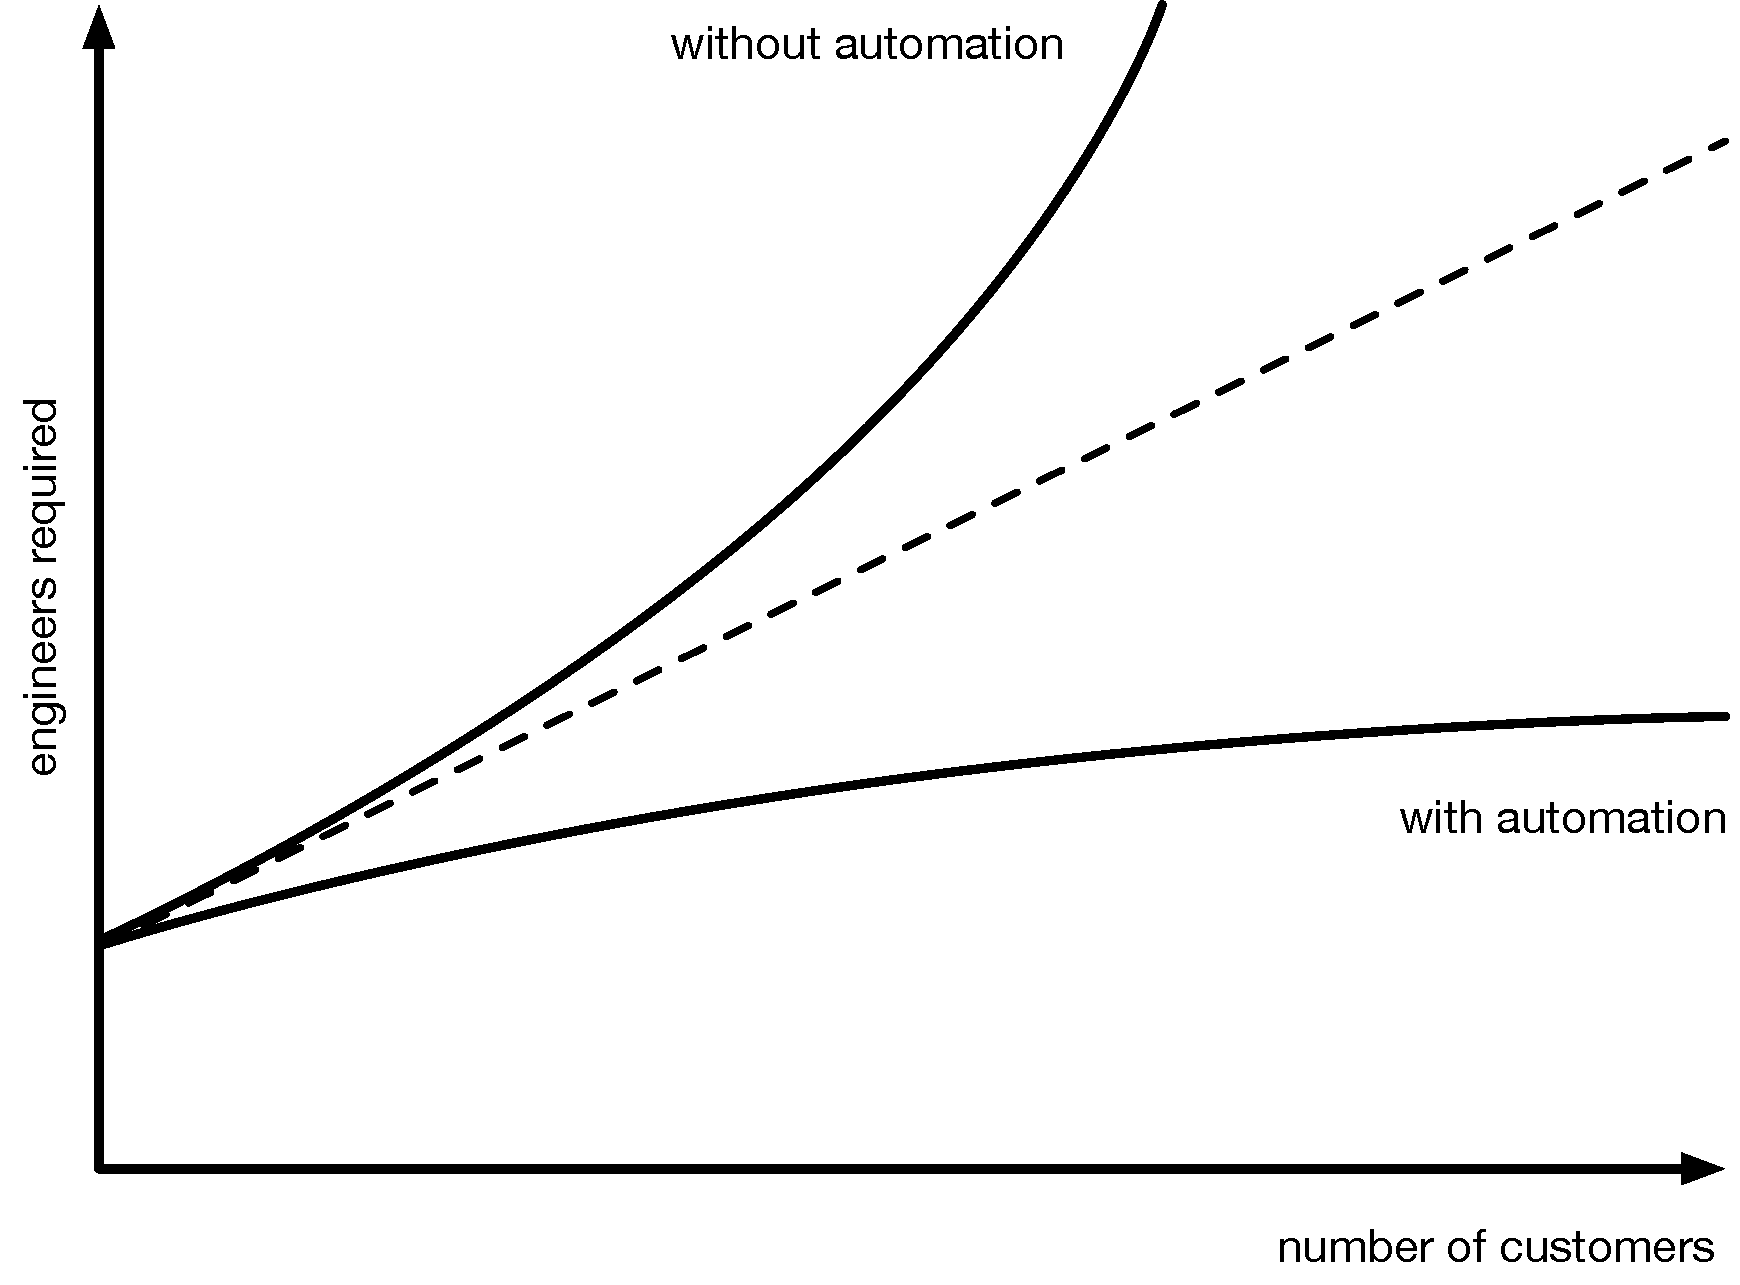
\includegraphics[width=1\textwidth]{figs/scaling}
		\caption{engineers per customer}
		\label{fig:engineers-needed}
	\end{subfigure}
	\begin{subfigure}{0.45\textwidth}
		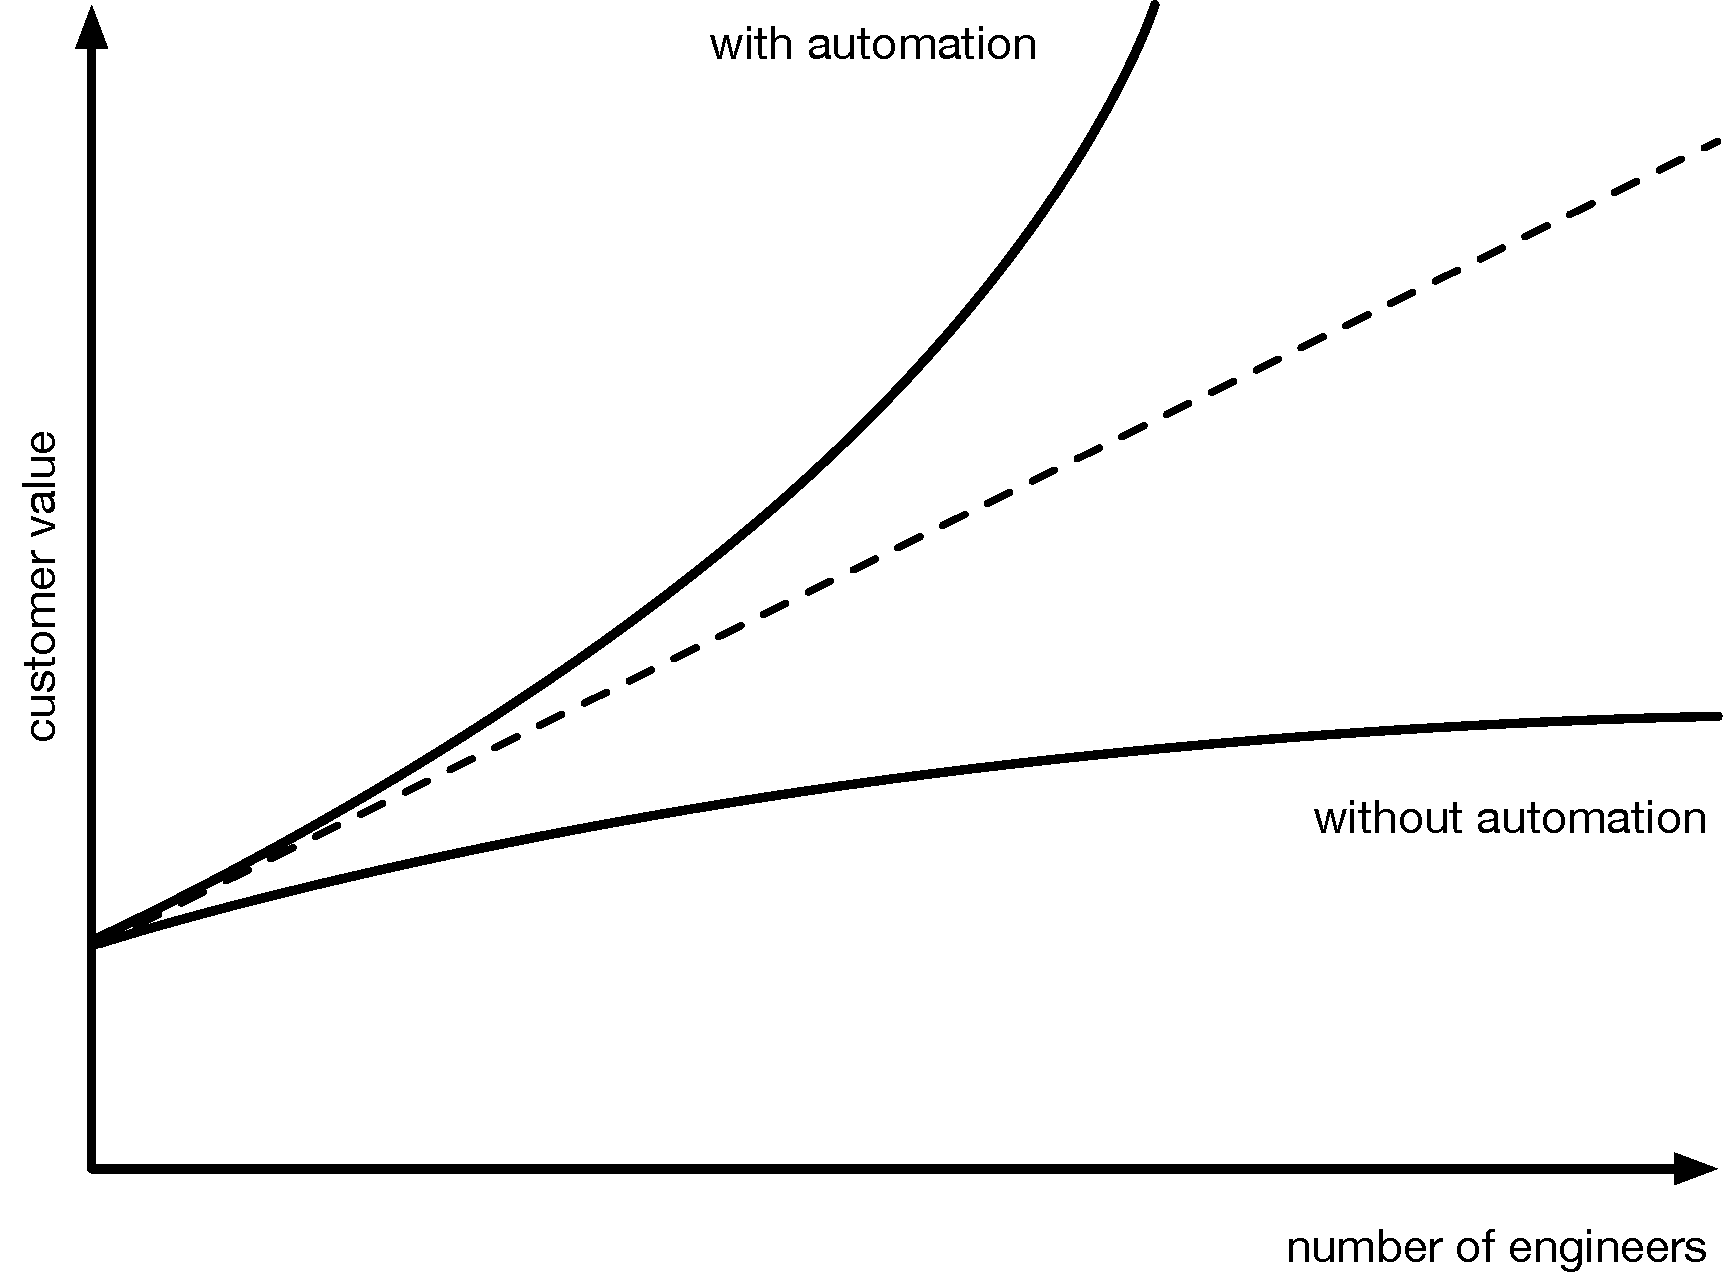
\includegraphics[width=1\textwidth]{figs/customervalue}
		\caption{customer value per engineer}
		\label{fig:value-engineer}
	\end{subfigure}
	\caption{Scaling customer service}
	\label{fig:scaling}
\end{figure}

With increasing level of automation, the number of engineers necessary to support a product grows significantly slower with growth in the number of customers using that product, compared to more manual solutions [ref to google SRE] (figure \ref{fig:engineers-needed}). As a corollary, with automation, the customer value delivered grows faster with the number of engineers (as more engineers add even more automation, boosting productivity even more), while without it, adding more engineers relatively quickly brings diminishing returns (figure \ref{fig:value-engineer}). Automation enables relatively small teams of engineers to run products relying on a complex infrastructure whilst supporting millions of customers [ref WhatsApp]This is one of the reasons start-up companies outperform large corporations: their resource constraints mean they are forced to invest in automation and smart solutions over adding more people, which in turn results in a much more efficient system. When we employ automation, we move the engineering effort higher up the value chain towards customer facing features.

Recent advances in technology, and commoditization of tools and infrastructure, have now closed the gap in automation to the point where the entire product platform from infrastructure provisioning to deploying complex orchestrations of containerised microservices onto clusters of servers can be easily fully automated and managed, evolved, tested and reused in the same way (and by the same team) as application source code.

However, automation does not only bring speed and efficiency. Every time an engineer makes a manual change to the configuration of a platform, the knowledge encapsulated in that change is lost. The reason for the change, the time, and the previous state of the infrastructure are all lost. By storing the change as code in a version control system, we have a permanent, irrefutable record of when, who, why etc. This not only provides an audit trail of everything the platform has been since it was conceived, but, more importantly, also accelerates the evolution of the platform because each change can build on top of the captured knowledge of previous changes.


\section{Product platforms as Code}
\label{sec:ascode}

Starting from the industry accepted practices and moving to more novel, recently introduced concepts, we can cover the types of automation and configuration that will together form a fully-featured product platform entirely defined as source code.

First, \textbf{pipelines as code} is a common approach in the industry. The Continuous Integration and Continuous Deployment automation is managed as code and stored next to the application code it is building, testing and deploying. This automation has obvious efficiency benefits and storing the configuration as part of the codebase means application and builds do not get out of sync and no extra authorisation process is needed to change the automation configuration. The CI/CD service becomes a simple runtime environment for build and testing tasks.

Second, \textbf{immutable infrastructure as code} enables automated, repeatable, reliable and fast infrastructure provisioning. All instances of infrastructure can be identical to the production environment. Since provisioning is automated, the infrastructure can be torn down and recreated within minutes. This lets us treat infrastructure as ephemeral, and allows us to update configuration by destroying and recreating, rather than modifying infrastructure in place, making it effectively immutable. This also means no access to servers is required, which simplifies configuration and increases security significantly.

With Docker, containerised \textbf{application builds} can also be defined \textbf{as code}. Running applications in containers has several benefits. First, containers are lightweight and provide resource isolation guarantees while running on the same underlying operating system. More importantly, with Docker, containers are stored and transferred as images of a standard shape.

A container is a unit of deployment agnostic of the underlying infrastructure and the technology stack used by the application inside it. This draws a very strong boundary between the infrastructure and the application. The images are described with Dockerfiles, recipes of creating images step by step, stored as code []. Docker images are formed of layers, which are immutable and content addressed (by a cryptographic hash of their content) []. These properties mean that Docker images can be built once and deployed on any infrastructure supporting Docker.

In order to support high availability and reliability guarantees, it is necessary to run applications across multiple computers, generally called a cluster. Operating a cluster is a complex task. Among other tasks, we need to manage nodes joining and leaving, make scheduling decisions, i.e. which instance of a particular service to put on which of the available nodes, supporting affinity and anti-affinity constraints while maximising the efficiency of resource usage, and manage automated scaling and failover. Cluster orchestration should also provide built-in service discovery, so that instances do not need to be aware of the layout of the cluster.

In recent years, cluster orchestration has been distilled into easy to use tools, which provide all of the features above out of the box, e.g. Mesos, Docker in Swarm Mode, Kubernetes, etc. These are generally based on a concept of control loops reconciling the current state of the cluster with the desired state, declared in the cluster configuration [ref]. This means the cluster can automatically respond to changes in the underlying infrastructure (e.g. a machine failing, load increasing) as well as changes in the desired state, e.g. a new version of a service being available. Constraints can be put on the reconciliation strategies (e.g. only one instance of a service can change at a time) resulting in gradual, zero-downtime upgrades.

An important consequence of the way modern cluster management software is configured is the ability to provide \textbf{service orchestration as code}, i.e. the state of the cluster is configured down to the desired microservices that should run on it and their names, number of replicas and deployment strategies. Coupled with service discovery, this makes it significantly easier to operate applications built with a microservices architecture.

Microservices provide numerous architectural benefits - they can be built, tested and deployed in isolation, independently evolved, scaled and replaced and generally provide great design flexibility. The downside is the complexity of building, testing and operating complete systems composed of many microservices. Testing and operating a monolithic application is very easy. It is built as a whole, deployed as a whole and tested as a whole and there is no risk of a part of it suddenly changing, breaking the whole. This property does not hold for microservices - by definition they come and go, their API contracts change and even knowing what exactly is running in a given runtime environment is often a difficult task.

With service orchestration captured as code, some benefits of the monolith come back. In essence we reify the service orchestration and gain a single entry point (a “handle”) into what the application consists of when running. There can be multiple sets of configuration for different environments, potentially adding or omitting certain services, configuring certain services differently (via environment variables), etc. All this information would normally be either lost or scattered across configuration files and deployment scripts.

With most cluster orchestration tools (e.g. Docker in Swarm mode, Kubernetes) sets of configuration, we will refer to them as “stacks” (a name used by Docker), can be deployed under an alias, which also forms a namespace for the services. Within the namespace, services can refer to each other by local names, making the entire stack portable, without any change of configuration. This gives a really light-weight mechanism of creating logical environments in a cluster.

As an added benefit, the service orchestration is immutable. In order to change the configuration or topology of the microservices, the code describing it is changed and the orchestration redeployed. The cluster orchestration system then reconciles the differences so that only the parts that are different actually change. Repeated deployments and updates are idempotent - if there is no difference, nothing changes. This declarative approach means we can logically treat the whole service orchestration as a single unit for deployment and let the automation handle the details. We show the specifics of making sure this property holds in Appendix~\ref{sec:architecture}.

In figure \ref{fig:concerns} we show 48 cross-cutting concerns, identified by Sean Treadway~\cite{Treadway17:online}, that need addressing for each microservice. None of them are directly related to adding customer value. With microservices architecture, we have made a rod for our own back: developers should be able to write code that directly adds customer value and they should not need to worry about any of the concerns listed. These can be addressed by employing a service mesh (such as Istio []). It allows us to declaratively specify \textbf{policy as code} providing services such as intelligent routing and load balancing, traffic shaping and shifting, security policies, ingress and egress rules, circuit breaking [] and upstream call retries, rate limits, call tracing, telemetry and reporting. It is even possible to use a service mesh to inject faults into the system to test reliability features that may have been overlooked. All of this configuration is declarative and stored as code alongside the orchestration configuration.

With microservice orchestration and policy being captured as code, the question arises as to whether or not to share microservice instances between application stacks. In other words, can each application have its own replica of the same microservice or should there be a shared instance? Notice this choice is only valid for stateless microservices, as when replicating microservices which hold state, data replication and distributed transaction concerns arise, which are typically hard enough to solve to warrant being solved once and only once. This difficulty should not be underestimated and it is often a good approach to try to split the microservice into its business logic and persistent data storage concerns and separate out as much of the stateless part of as possible, e.g. by using a Database as a Service (DbaaS). The business logic then becomes a separate, now stateless, microservice.

For truly stateless microservices, it is simpler if each of the applications has its own copy of a microservice treating it simply as a module of the system, re-using and sharing only its source code. In order to share a microservice instance, it needs to be fully treated as a service, as it is no longer under the control of the team managing the application - it essentially becomes a 3rd party dependency. In that case, it should have an agreed service level, support model, documentation, versioning and migration strategy, etc.

In a sense, there are two levels of reuse: microservices, reusing the code, where operations fall under the same team as the rest of the application, and services, reusing the instance as well, where the ownership is more complex and coordination is necessary.

\section{Microplatforms}
\label{sec:microplatforms}

Building on everything from the previous sections, we can now give some clarity to the term Microplatforms, that we use to refer to the model of runtime environment management we describe in this paper.

The key feature of Microplatforms is not technical, it is organisational - the concept of product team autonomy. This is important, because all of Engineering can (and should) be answerable to Product (ultimately customers) rather than Technology. Technology is a means to an end, an enabler, a multiplier. Autonomous cross-functional teams can leverage technology to meet the product demands of the customer. Infrastructure automation is what enables them to do so.

Consider the diagram from figure \ref{fig:automationn} again, this time with infrastructure approaches and technologies superimposed on the spectrum (figure \ref{fig:automation-techniques}). With the currently available level of automation, it is now entirely possible for a cross-functional team of ten to operate a fully-featured product platform for their application. This level of vertical integration has numerous benefits.

It removes the coordination cost of all product teams depending on a single platform team. If a team needs to change some aspect of their platform or add a missing feature, they can do so for themselves. A platform team will most likely still exist, but the product it delivers is the design and automation of a platform, not the infrastructure itself. This team can become an owner and steward of the platform design, which can and should be internally open source, so that everyone can contribute and the platform engineers can transition into expert support and innovation roles, rather than day to day operations. This is a tried and tested approach which works well for shared, reusable code libraries and services []. With the shared dependency removed, the organisation becomes more horizontally scalable, just like software systems do. Vertical integration leads to horizontal scalability.

\begin{figure}[h]
	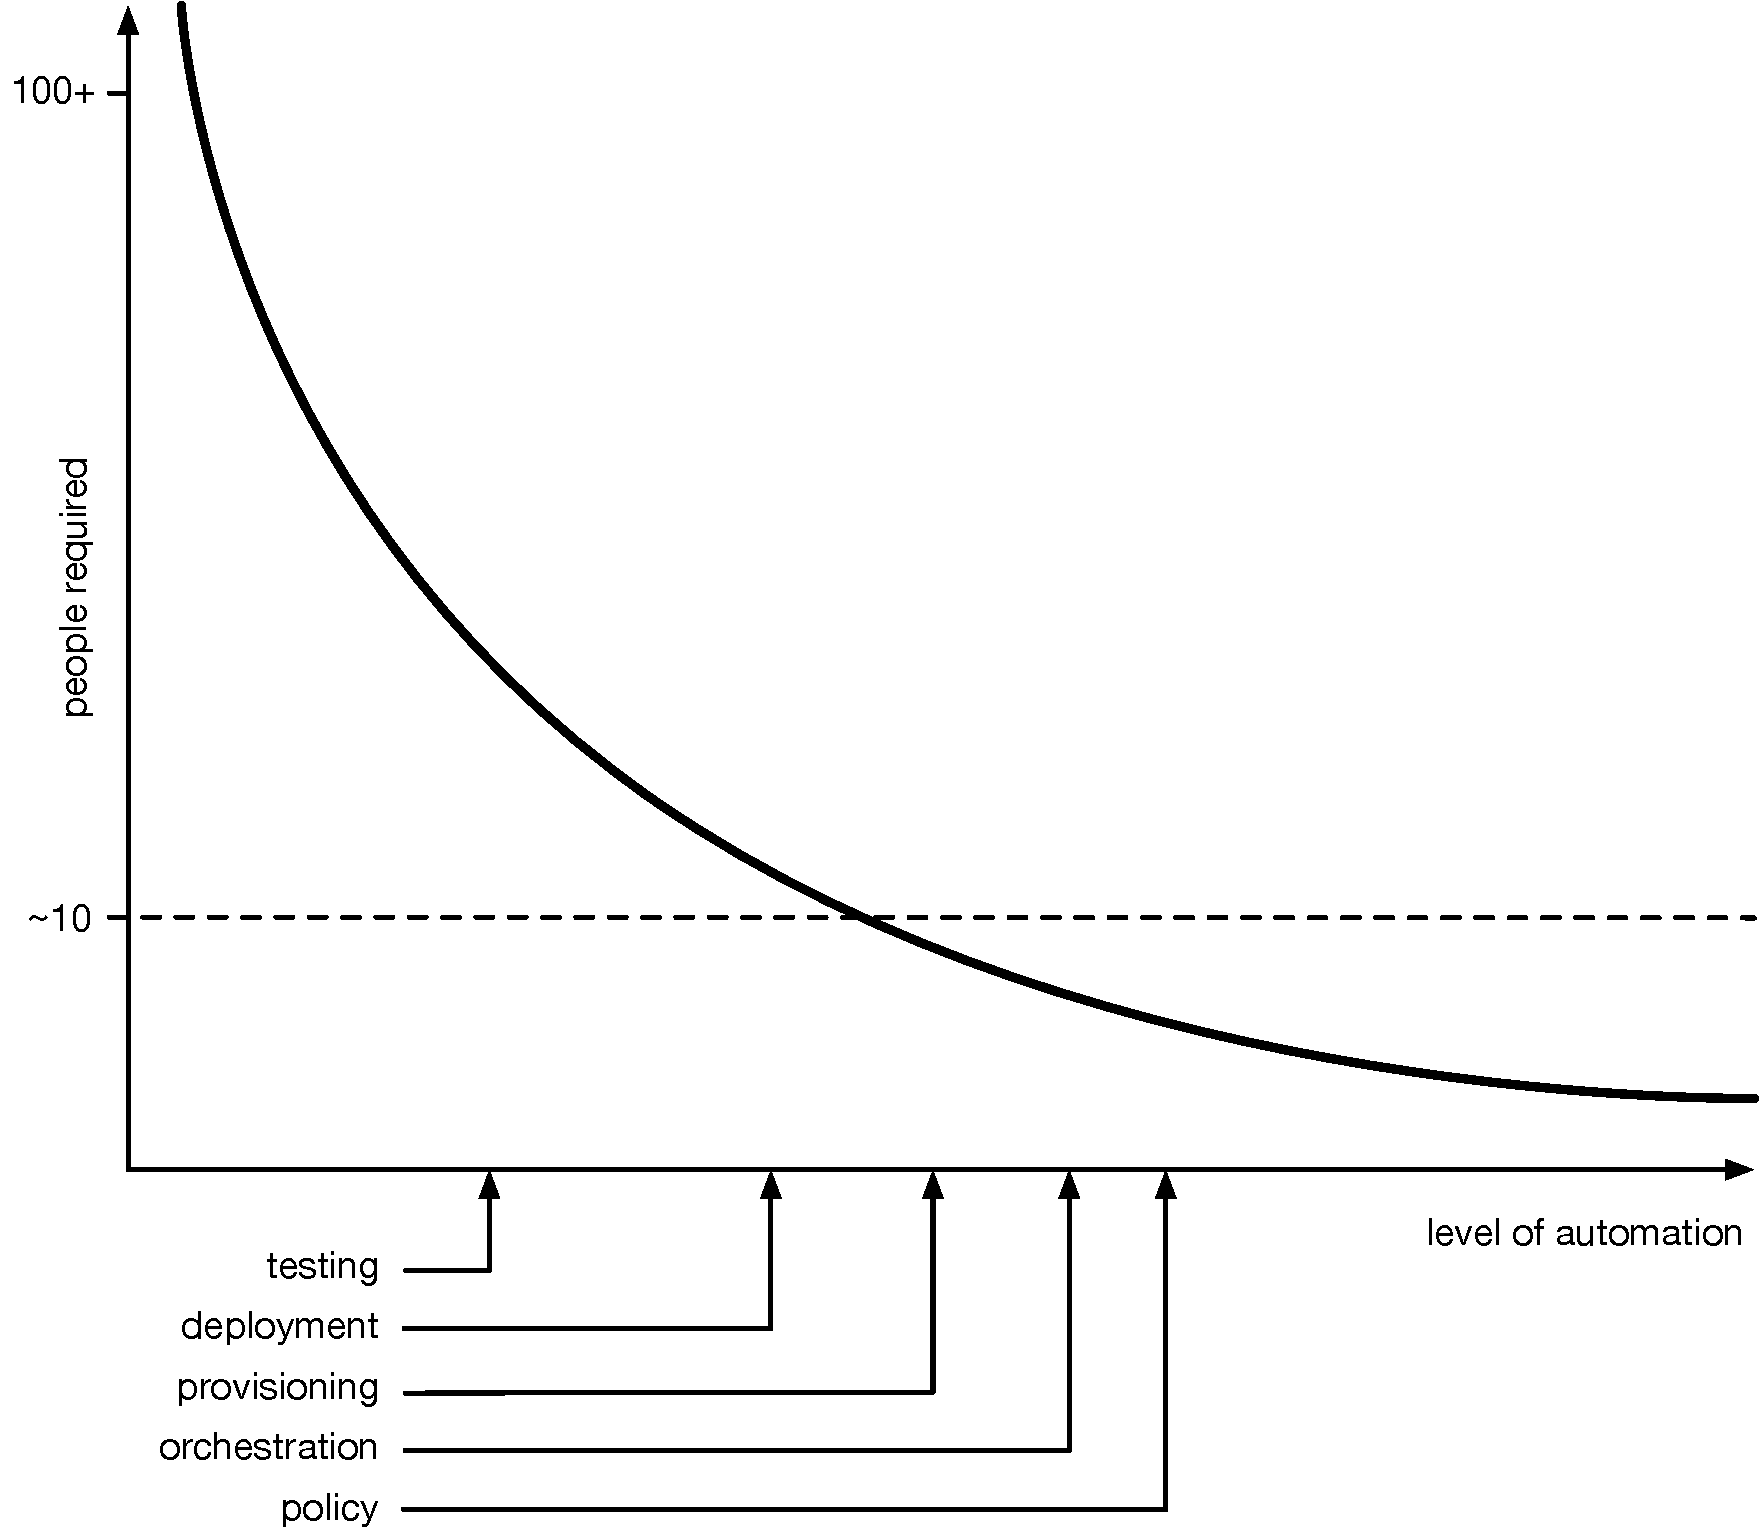
\includegraphics[width=0.45\textwidth]{figs/automation-tools}
	\caption{Automation techniques}
	\label{fig:automation-techniques}
\end{figure}

Small separate platforms also provide a much smaller blast radius in case things go wrong. On a shared platform, a lot of effort needs to go into preventing cascading failures caused by one application overloading a shared resource and in turn causing a different bottleneck to cause more failure. Isolation features like this are a case of multi-tenancy support, which needs to be built into a shared product platform. This can be completely omitted from a Microplatforms based design.

Shifting all the design, management and reuse towards code enables Agile Architecture and a degree of diversification to fit individual product’s requirements without ending up with either a superset of all the features or the least common denominator that works for nobody. This also opens the platform up to a free competition of ideas leading to continuous innovation without big, dedicated innovation budget.

The fully automated provisioning, operations and deployments enable provisioning separate, ephemeral platforms for various purposes (e.g. performance testing or penetration testing). In an extreme case, all environments could be ephemeral and only exist for hours or days, with the exception of the live production one, but even the production environment can be regularly rebuilt in a blue-green fashion []. As a byproduct, this facilitates natural slipstreaming of software upgrades and security patches (by using the latest stable version of the software) that would otherwise have to be specially considered.

Targeting a cluster orchestration technology, applications become fully portable between any infrastructure supporting the technology from a developer’s laptop through any public cloud provider to on-premise solutions. Kubernetes [] is rapidly becoming a de-facto standard in cluster orchestration: it is possible to run a local cluster using a tool like Minikube [], clusters can be provisioned using simple compute resources in different clouds with Kops [], all three major cloud providers are offering or have announced hosted services (GKE [], EKS [] and AKS []) and managed on-premise solutions also exist, e.g. OpenShift by RedHat []or Pivotal Kubernetes Service [].

Finally, the level of automation required for a small platform to be managed by an average sized product team enables a capability crucial to agile software delivery: continuous deployment to production. With continuous deployment to production, every change to the application and infrastructure goes through thorough automated testing and validation. Once the validation passes without issues, the change is deployed to production. This can happen several times a day, even multiple times an hour.

This sounds really risky at first, but consider that as the time between deployments tends towards zero, the size of the change also tends towards zero and the risk that change carries also tends towards zero. If things go wrong after a particular deployment, it is trivial to understand the cause of the problem, because the set of causes to consider is minimal. The age of the change deployed tends towards zero as well, and since it was made very recently, it is fresh in everyone’s heads which makes it much easier for them to understand the possible causes.

Continuous deployment to production also enables the practice of “fixing forward” rather than rolling back to a likely safe state. Both techniques are still relevant, but the ability to quickly and reliably fix forward becomes important when a problem is discovered after some time has passed. We consider a special process for deploying a hotfix an anti-pattern to be avoided: hotfixes should be deployed through the same process as any other change. Because hotfixes are relatively rare, the special hotfix process is not executed very often and is more likely to fail, which is the worst problem to face when trying to fix an urgent production issue.

With continuous deployment to production, it is necessary to decouple deployments from customer releases, via a mechanism like feature flags, which bring a benefit of decoupling the engineering process of deployment from the business process of customer release. The control of feature release can even be directly given to the product owner.

Altogether, the reduction in coordination cost, the automation of provisioning, continuous integration and deployment, increase in reliability and availability and mean time to recovery from incidents adds up to a significant amount of time which can be invested into innovation and, most crucially, delivering value to customers.


\section{\label{sec:simplicity}Simplicity as the guiding principle}

We have shown how several main principles contribute to overall efficiency of the Microplatforms concept. We will now attempt to tie these together with a single guiding principle of design we believe leads to the most robust, efficient and future proof solutions.

The first overarching principle is automation, in other words committing decisions and processes to code. This means designs and processes can evolve over time, are repeatable, easy to adopt, specifications are precise and complete and with version control systems, history does not get lost. This enables us to keep all instances of infrastructure and automation perfectly aligned, simplifying the overall result. Automation also allows as many things as possible to become immutable.

Immutability, i.e. preventing things from being updated in place implicitly creates a version history of all changes and makes it impossible for anything to change unexpectedly or get into a certain state in any other way than being recreated. Removing previous versions of things is a case of garbage collection to reclaim resources they consume. Immutability decouples values, i.e. the entities (infrastructure, build artifacts, deployments, etc.) from the identities, the way we refer to them over time, e.g. “the customer service”. [Rich Hickey]

Immutability is typically quite easily attained by content addressing - referring to any data by a cryptographic hash of the content itself. This concept appears a few times in our approach: code stored in git is referred to by the sha1 hash of the contents of a given revision [], Docker images and layers can be immutably referred to by a \texttt{sha256} hash of their content [].

With immutability and with content addressing especially, it is much easier and efficient to compare two items of the same type (i.e. just by their names), enabling idempotence: the concept of actions which can be repeated many times producing no further result beyond the first application. Enabling easy idempotence leads to huge simplification, as we can typically stop focusing on detail and let idempotence handle the unwanted repetition. In a sense, idempotence unifies creation and update and makes both operations the same from outside, moving solutions from imperative to declarative. We can say that idempotence decouples intent from current state. This also appears multiple times: infrastructure provisioning with Terraform, Docker image builds and pushes to registry, deployment to a cluster or response to failure with the reconciliation loop. Everything tries to reach a declared state.

The third major principle is autonomy. In organisations, autonomy removes coordination costs, confusion, bottlenecks and queueing which leads to politics. From a systems perspective, lack of autonomy is a form of coupling. In software engineering, unnecessary coupling is understood to be a problem []. An interesting case of coupling is sharing and reuse, typically seen as purely beneficial without considering the cost.

All of the above - automation, immutability, idempotence and autonomy are cases of simplicity, \textit{simple} being distinctly different from \textit{easy} [simple made easy]. By simple, we mean having a minimum of structure, little coupling and entanglement, avoiding N:M relationships between entities. Immutability is also a case of decoupling - mutable state is one of the hardest to understand couplings - a coupling through time.

The chief guiding principle in every decision made when designing a product platform should be to try to minimise complexity above everything else. This, in our opinion, extends to all software engineering, as the human capacity for understanding complexity is the biggest limiting factor of the systems we design and build.

\section*{\label{sec:summary}Summary}

Repeat the 5 things that enable Microplatforms
Repeat the 3 process/engineering approaches that Microplatforms
Go through how this applies to the goals stated in the introduction

\newpage
\clearpage
\appendix
\section{\label{sec:architecture}Microplatform Reference Architecture using Kubernetes}

A microplatform reference architecture should describe everything that is required to be able to create and configure identical microplatforms, on any provider (including laptops, on-prem and cloud) in minimal time and with minimal effort (i.e. as fully automated as is possible). This includes sample code that actually works and all the associated documentation needed to quickly grok the system, so that an individual, who may be new to both the concepts and the implementation, can get immediate value.

A reference architecture does not represent a fully evolved or production-ready state, but may well be used to model an implementation that does.

\bibliography{bibliography}
\bibliographystyle{plain}

\end{document}
%
% ****** End of file apssamp.tex ******
